\chapter{Modelization of central perpspective cameras}


%-----------------------------------------------------
%-----------------------------------------------------
%-----------------------------------------------------

\section{Introduction}

In this chapter we introduce the mathematical model used in {\tt MMVII}
for modelization of central perspective camera.  The majority (if not all)
of images we manipulate in current life are acquired by central perspective camera, it includes
smarthphone cameras,  reflex cameras,  most aerial cameras \dots  In fact they are so common that
it is easier to define camera that are not central  perspective :
it include majority of satellite images and few aerial camera (like leica-ADS40).

We start from the most basic model and introduce progressively different refinement,
being cautious to justify by physic considerations all the parametric terms we introduce.
We also introduce the convention selected in {\tt MMVII} as in photogrammetry/computer vision
there are several arbitrary choices that may be confusing.

%-----------------------------------------------------
%-----------------------------------------------------
%-----------------------------------------------------

\section{Camera Obscura and  central perspective model}

%-----------------------------------------------------
\subsection{Physicall model}

\begin{figure}
\centering
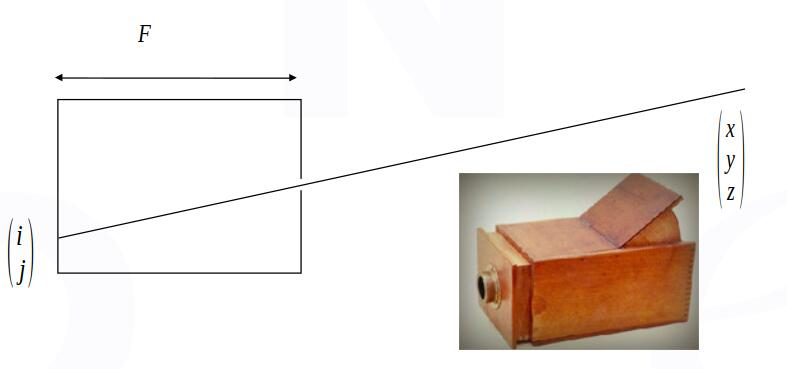
\includegraphics[width=12cm]{Methods/Images/CameraObscura.jpg}\caption{Camera osbcura : schema and a real object}
	\label{fig:CameraObscura}
\end{figure}


We begin by the description of very simple object, but which is really a the origin of
the photography and, in some way, is the simplest possible camera  :  the camera obscura.
Basically it can be described as a box with a hole, at the entrance of the box we have
a the hole that let the light in, and at the bottom of the box we have the film of
the camera. 

Figure~\ref{fig:CameraObscura} presents a real camera and a basic schema showing
the construction of the image :  to compute the image of a point $P^c=x^c,y^c,z^c$ of the real scene
we juts have to trace the line starting from $P^c$, going throw the hole and take its intersection $q=i,j$
with the image plane.


%-----------------------------------------------------
\subsection{Setting equations}

To compute a mathematical relation between $x^c,y^c,z^c$ and $i,j$ we will introduce several hypothesis 
and notations illustrated by figure~\ref{fig:Camera3DNote} :

\begin{figure}
\centering
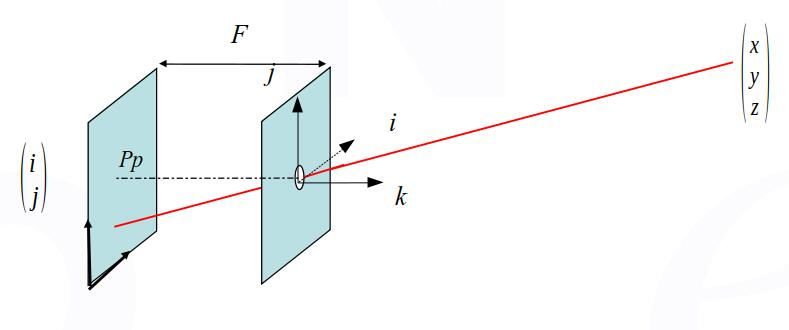
\includegraphics[width=12cm]{Methods/Images/Camera3D.jpg}\caption{Notation for camera relation}
	\label{fig:Camera3DNote}
\end{figure}

\begin{itemize}
	\item for 3d coordinates, we consider a local $3d$ repair $(O,\vec{i},\vec{j},\vec{k})$  where $O$ is the entrance hole,
              $\vec{i},\vec{j}$ belongs to the image plane and $\vec{k}$ is orthogonal to  $\vec{i}$ and $\vec{j}$;

	\item for $i,j$ we consider a image repair originated at one corner $c$ of the box;

	\item we note $P^p$ (principal point)  the intersection of axe $O\vec{k}$  with the image plane,
	      and $F$ (focal length) the distance between $P^p$ and $O$.

        \item we note $Q_3$  the $3d$ point corresponding to $q$.

\end{itemize}

To compute coordinates of $Q_3$ we can use chasles relation as indicated in equation~\ref{PC:Chasles} :

\begin{equation}
	\overrightarrow{OQ_3} =  \overrightarrow{O P^p} + \overrightarrow{P^p c} +  \overrightarrow{c Q_3}
	 =     \begin{pmatrix} 0\\0\\-F \end{pmatrix}
             + \begin{pmatrix} -P^p_x\\-P^p_y\\0 \end{pmatrix}
             + \begin{pmatrix} i\\j\\0 \end{pmatrix}
	 =     \begin{pmatrix} i-P^p_x\\j-P^p_y\\-F \end{pmatrix}
	\label{PC:Chasles}
\end{equation}

Now remind that light having a straight path, the $3$ point $Q_3$, $0$ and $P^c$ must be aligned,
which can be wrotten by equation~\ref{PC:Alignment} :

\begin{equation}
	\exists \lambda : 
	\begin{pmatrix} i-P^p_x\\j-P^p_y\\-F \end{pmatrix} 
      = \lambda   \begin{pmatrix} x^c\\y^c\\z^c \end{pmatrix}
		\label{PC:Alignment}
\end{equation}

By a simple quotient  we can elimimnate $\lambda$ in~\ref{PC:Alignment} and obtain :


\begin{equation}
	i = P^p_x -F \frac{x^c}{z^c}  \; ; \;
	j = P^p_y -F \frac{y^c}{z^c}  
	\label{PC:FormulaImaIntr1}
\end{equation}

%-----------------------------------------------------
\subsection{Local image formula}

The usage is to modiy the equation~\ref{PC:FormulaImaIntr1} by changing the sign of $F$;
this comes to consider a camera model ,
 not physically feasible and slightly different from the camera obscura,  
where the image plane is before the whole instead of behind, and that
is illustrated by figure~\ref{fig:PcInvCam}.  

\begin{figure}
\centering
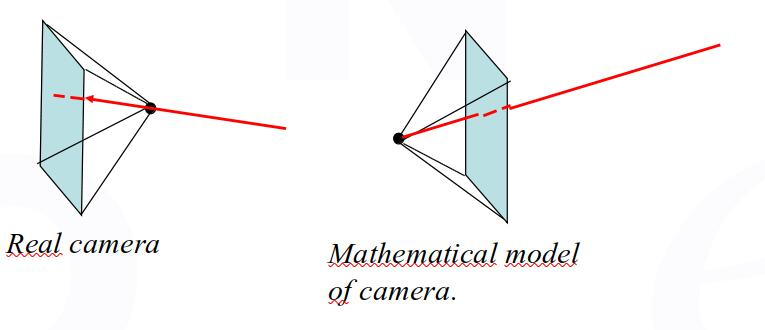
\includegraphics[width=12cm]{Methods/Images/InvCamera.jpg}
	\caption{Camera model : physically based one (left) and used one (right)}
	\label{fig:PcInvCam}
\end{figure}

Finally we will use equation~\ref{PC:FormulaImaIntr2} to formulate the relation between
local ground coordinates $P^c$  and image coordinate for this basic camera :

\begin{equation}
	i = P^p_x +F \frac{x^c}{z^c}  \; ; \;
	j = P^p_y +F \frac{y^c}{z^c}  
	\label{PC:FormulaImaIntr2}
\end{equation}

Setting the canonical projection $\pi_0$:

\begin{equation}
	  \pi_0 \begin{pmatrix} x^c \\ y^c \\ z^c \end{pmatrix} 
           =  \begin{pmatrix} \frac{x^c}{z^c} \\  \frac{x^c}{z^c}  \end{pmatrix} 
\end{equation}

and the intrinsic calibration $ \mathcal{I}_0$ :

\begin{equation}
	   \mathcal{I}_0  \begin{pmatrix} u \\  v  \end{pmatrix} 
		   =  P^p + F  \begin{pmatrix} u \\  v  \end{pmatrix}  \label{EqIntNoDist}
\end{equation}

we will write :

\begin{equation}
	q  =   \mathcal{I}_0 (\pi_0 (P^c))
\end{equation}


%-----------------------------------------------------
\subsection{Global image formula}

Generally we need to write the coordinate of $q$ as a function of the global coordinate $P$ or a point.
For this we just have to write the local coordinates $P^c$ as a function of global $P$, 
we use $C$ the center of the camera, and $R$ its orientation :

\begin{equation}
	P =  C+ R *P_c
\end{equation}

Which give the image formula :
\begin{equation}
	q  =   \mathcal{I}_0 (\pi_0 (^t R (P - C))) \label{FormImage0}
\end{equation}

This formula will follow us for a long time. The main thing that will evolve is $\mathcal{I}_0$,
and later $\pi_0$,
that will become more sophisticated to take into account lenses used in real camera.


%-----------------------------------------------------
\subsection{A remark on repair orientation}

We have not discussed untill now which image repair is used for image coordinates $i,j$.
The choice done in {\tt MMVII} is to use the native coordinate system of the image format,
knowing that majority of image format use a clockwise repair : 
that is : $i$ is left to right and $j$ is up to bottom (this is purely conventionnal, but one the
choice is made, is will have to be respected all along the process).

As we aline  local repair $(O,\vec{i},\vec{j},\vec{k})$  on this coordinate system ,
and we want a direct $3d$ repair with $\vec{k} = \vec{i} \wedge \vec{j} $, this
has for consequences that with these convention the axe $O\vec{k}$ is in the viewewing direction of the
camera.  The figure~\ref{fig:FormIm} illustrates this convention;


\begin{figure}
\centering
	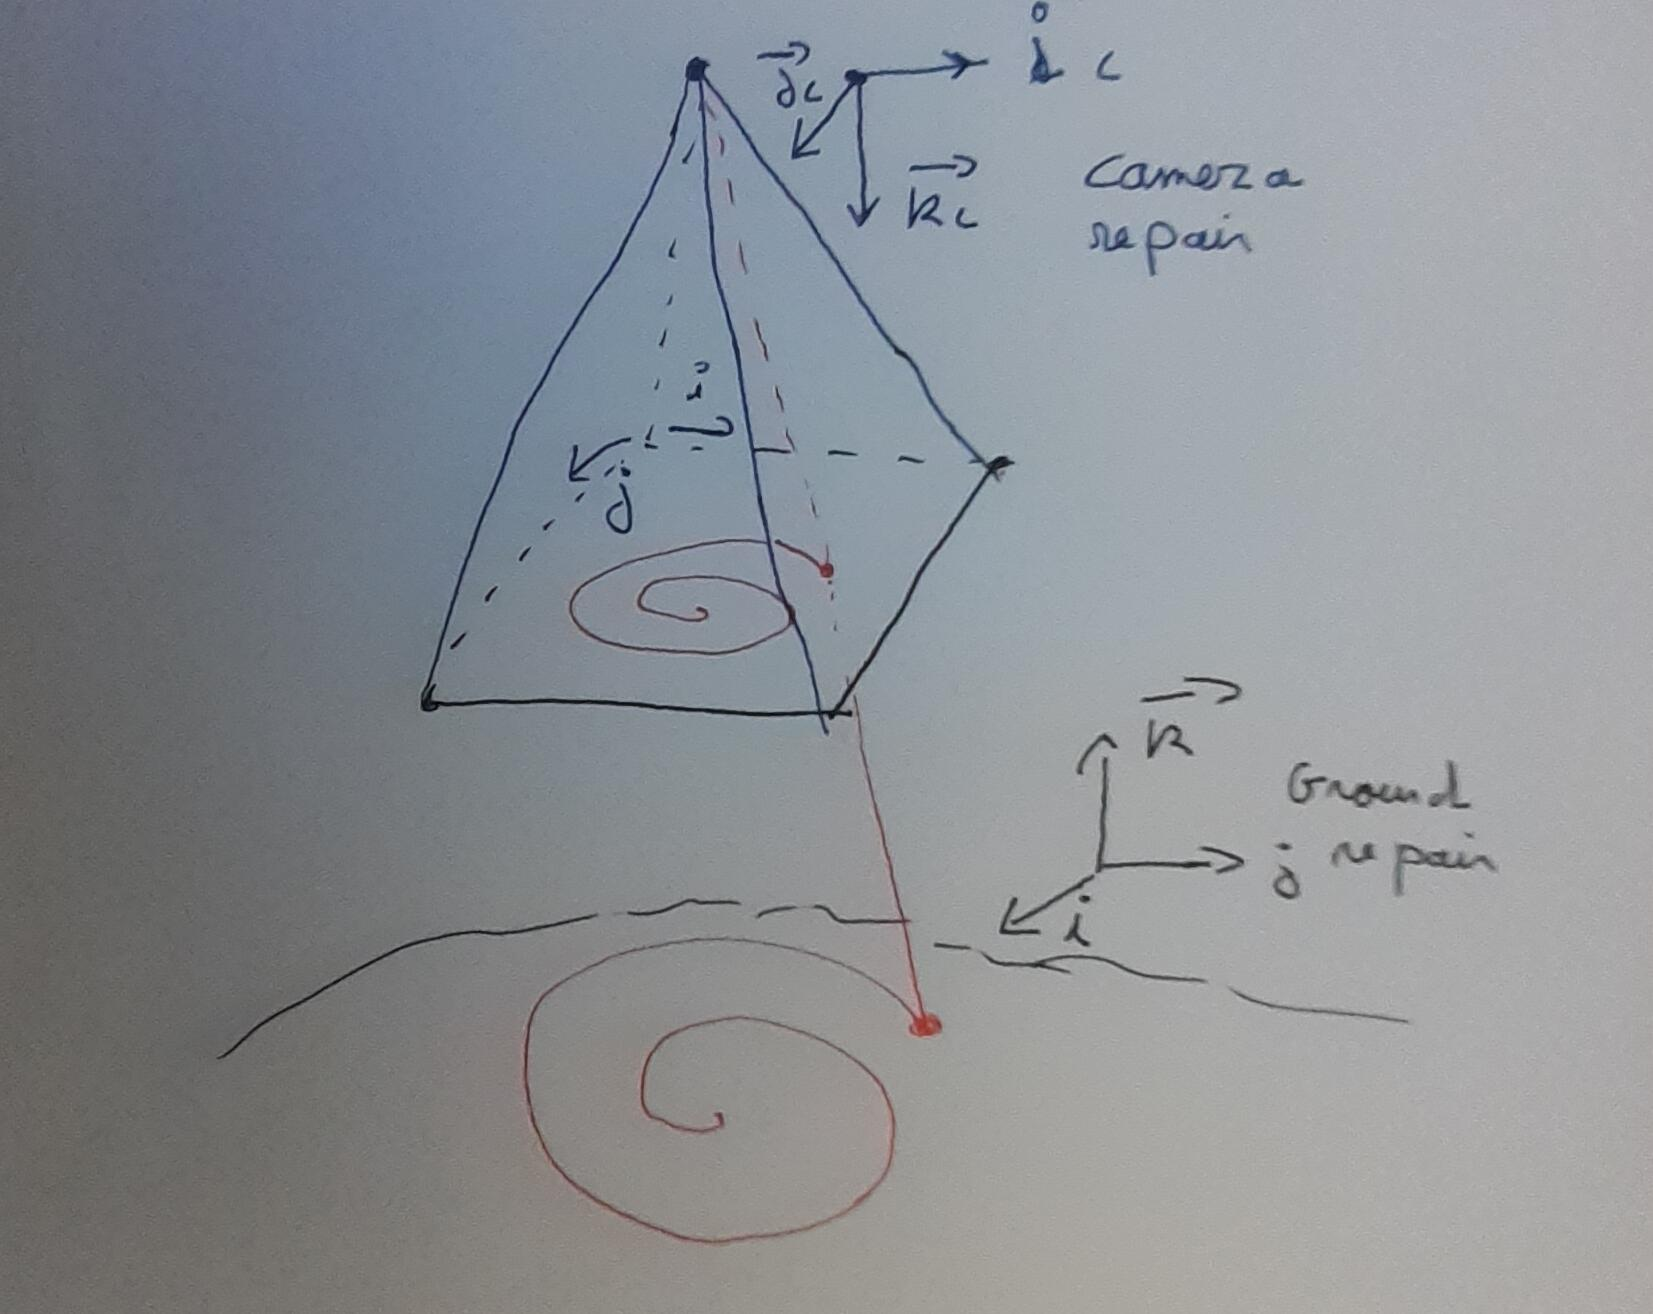
\includegraphics[width=12cm]{Methods/Images/RepairCam.jpg}
	\caption{Camera model : physically based one (left) and used one (right)}
	\label{fig:FormIm}
\end{figure}

%-----------------------------------------------------
%-----------------------------------------------------
%-----------------------------------------------------

\section{Beyond camera obscura}

%-----------------------------------------------------
\subsection{Need of lenses}

With the camera obscura, to have a sharp image we must keep a small entrance hole;
so to have enouh light we need very long exposure time (several hours). 
This is not convenient and the devlopment of photography
would not have been possible without the devlopment of optic. By puting a system
of lenses at the entrance of the system, and being caution that the  scene focalise
on the image plane, it was possible to have a sharp image whith a sufficiently big
hole and make photography practicable.

Nowday all the camera have more or less complicated system of lenses. In fact due the
automatization of the computer added conception they tend to be more and more complex, the concepter
using the possibility offered by multiple lenses with various materiel to correct more and more optical defaults .

For photogrammetry it change the game, because the lenses being not "infinitely thin", the gauss
condition non longer apply and some non linearity will occur , we will no longer be able to use
equation as simple as~\ref{EqIntNoDist} and will have to modelize accurately the effect of
lenses. 


%-----------------------------------------------------
\subsection{A parametric estimation issue}

A possible way to proceed would be to take into account the CAD plane of the optical
system, use in conception and to deduce the correction using the law of optic.  
Practically, we almots never proceed this way for two reasons  :

\begin{itemize}
   \item firt this CAD plane are rarely avalaible (maybe due to industrial property ?);
   \item second, and more important, the experience prove that when we proceed to the
         modelization of two lenses from the same model, we have to modelize them with two
         different parameter if we want to get the best accuracy, so no theoreticall model 
         would fit our requirement (also it could give a good first approximation);
\end{itemize}

So the approach currently used in photogrammetry is to select a parametric model
for the effect of lenses and to estimate the paramaters from the measures we have  (tie-point,
GCP, GNSS  \dots).


%-----------------------------------------------------
\subsection{Precaution to take}
\label{ParamFit}

\begin{figure}
\centering
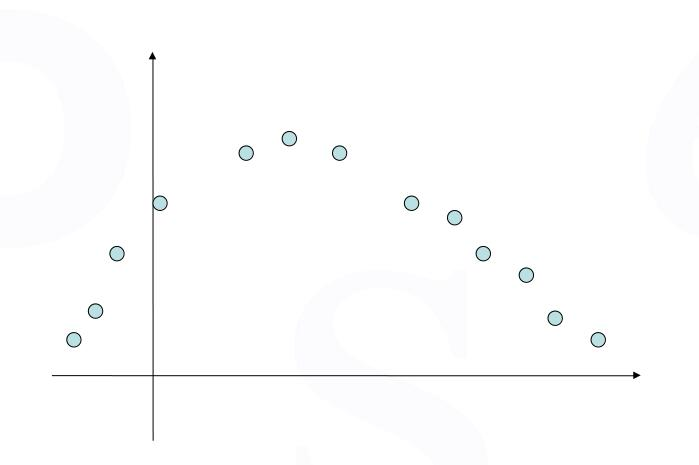
\includegraphics[width=6cm]{Methods/Images/Courbe-Pts.jpg}
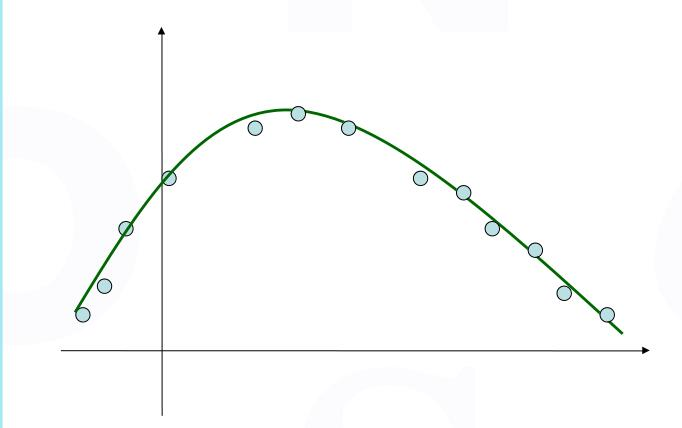
\includegraphics[width=6cm]{Methods/Images/CourbeGoodParam.jpg}\\
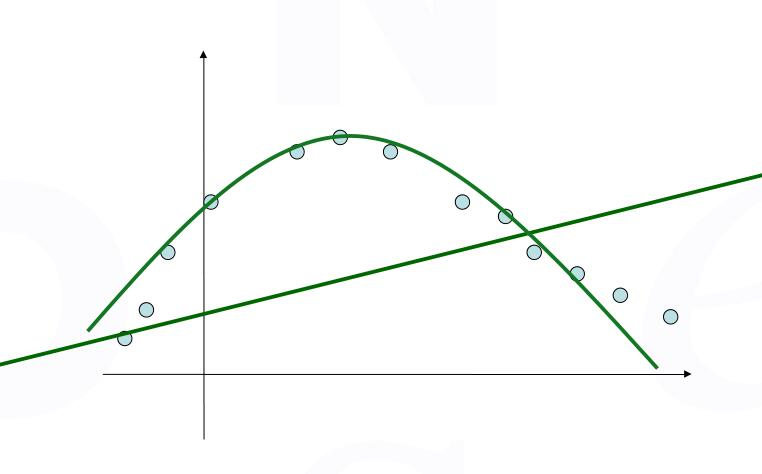
\includegraphics[width=6cm]{Methods/Images/Courbe-UndeParam.jpg}
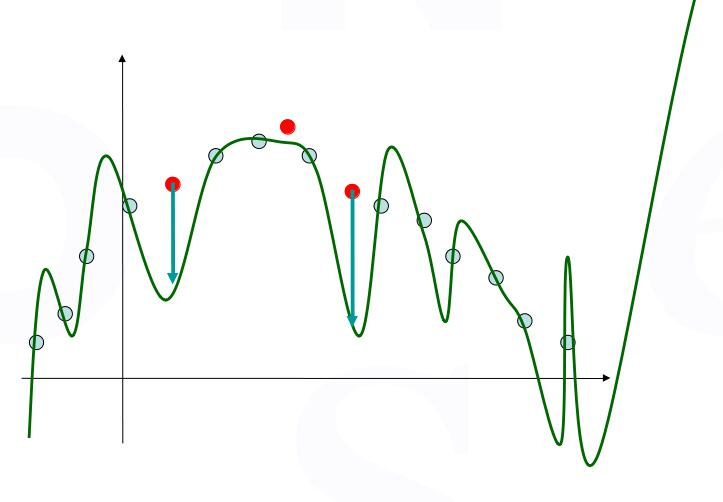
\includegraphics[width=6cm]{Methods/Images/CourbeOverParam.jpg}
	\caption{(1)Curves to interpolate (2) "Good" parametrization (3) Under parametrization (4) Over parametrization}
	\label{fig:CurvesParam}
\end{figure}


This empiricall approach does not prevent from being cautious
to the selection of model, we will have the usual compromise in the selection
of the parametric model, illustrated by figure~\ref{fig:CurvesParam}  on a problem of curve interpolation:


\begin{itemize}
	\item if we don't have enough parameters (curve 3) we are not accurate  even on the data to fit,
	   here if we fit with a straight line, or even with a parabol, we are not close to the learning data ;

   \item if we  have too many parameter (curve 4), we can have a very good match on the learning data, but have 
	 poor result as soon as we test with new data; this illustrated with  figure ??? were
         we use the "naive" lagrange interpolation to fit $N+1$ point with a $N$ degree polynomial,
         we have a perfect fit and the learning data, but due to high frequences a very poor fit outside;
\end{itemize}

The question of selecting the adequate model is a difficult one, and to our best knowledge
still open in photogrammetry.  Is it preferable to have over or under paramatrization ? There
exists controvorsery arguments :


\begin{itemize}
   \item  on one hand, as illustrated by figure ~\ref{fig:CurvesParam}, on can argue that under parametrization is less dangerous
         than over parametrization;

   \item  on the other hand, in "modern" photogrammetry the measurement comes more and more from automatic system,
          we can easily have several ten thousands of tie points, so one can argue that there is no real risk to have $100$ parameter
          even when we only really need $10$.
\end{itemize}

Consequently, it was thought, that the best we can do in {\tt MMVII} is to offer a sufficient large set of model
of camera, from the simple ones to the most universal one, and let the user select them according to
the precise knowledge of his domain. 

\begin{figure}
\centering
	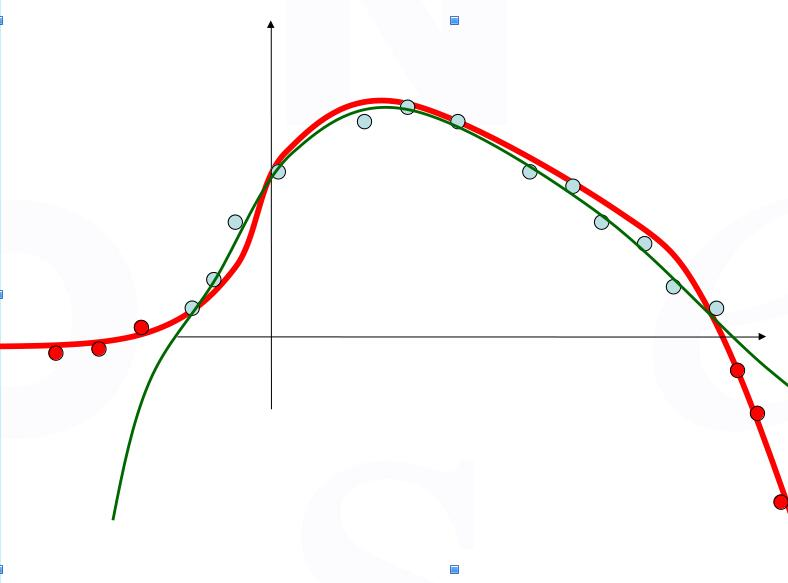
\includegraphics[width=6cm]{Methods/Images/CourbeExrapol.jpg}
	\caption{Extrapolation}
	\label{fig:CurvesExtrpol}
\end{figure}

However, even is this choice of parameter is not easy, there is
one universal rule : if we can be stable in interpolation, we are always bad in extrapolation
as illustrated on figure~\ref{fig:CurvesExtrpol}. A 
consequence when will estimate the model of a camera : if we have no measurement in the corners,
we are almost sure that we estimation will be poor in these corners.

%-----------------------------------------------------
\subsection{Still a central perspective, with a distorsion}
\label{Still:Persp}

In the next section we are going to introduce step by step, different model with a continuous
refinement of the physical modelization.  

\begin{figure}
\centering
	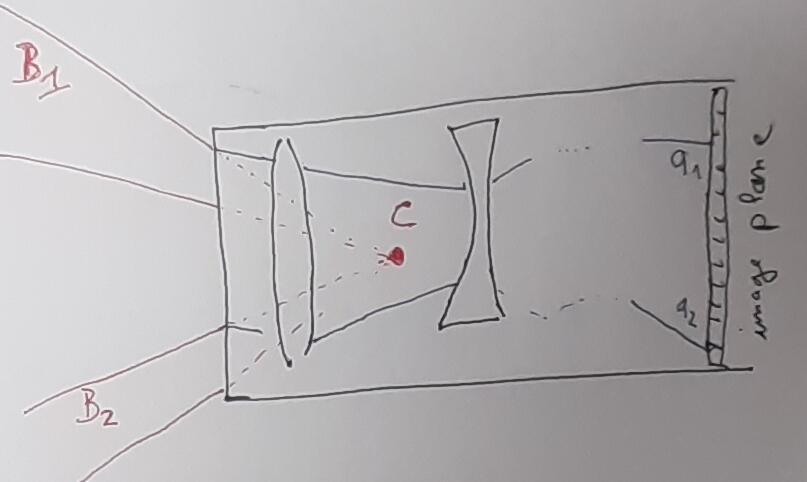
\includegraphics[width=8cm]{Methods/Images/CamPersp.jpg}
	\caption{Ligth path, all outing bundle converge to $C$}
	\label{fig:CamPerspScheme}
\end{figure}

The only hypothesis that we will maintain all allong these pages is that all the bundle issued from image
plane go through the same point $C$. This is schematised by figure~\ref{fig:CamPerspScheme} :
how complicated may be the ligth path inside the camera, we still have the property that
it exist a virtual point $C$, such that for any image point $q_i$, the bundle $B_i$ that lead to $q_i$
all go trough $C$.

This hypothesis is universally adopted, and justified because we still have a diaphragam that physicall contraint
the light to go trough it centers; of course the light will cross lenses before converning to this diaphragm but, 
, under gaussian approximation the image and reciproc image of converging bundle are still converging bundles.
To our knowledge, the only practicle cases where this hypothesis may be questionned are macro-photogrammetry and
sub-marine photogrammetry. We will discuss that ???. And maybe in the future of {\tt MMVII} project we will 
test option to relax this hypothesis for these context.

With this hypothesis, the image formation equation~\ref{FormImage0} still holds if
we add a supplentary $2d$ image deformation. Suppose in the initial simplistic camera
obscura, or even in a camera lenses satisfying gaussian approximation, 
the bundle $B_i$ would have arrived in $q^0_i$, now with the not thin lenses ,
it really arrive in $q_i$, we call $\phi$ the $2d$ mapping such that $\phi : q^0 \rightarrow q$.
With $ \mathcal{I}(q) = \phi (\mathcal{I}_0(q))  $, we have now :


\begin{equation}
	q  =   \mathcal{I} (\pi_0 (^t R (P - C)))
\end{equation}

By the way, for technicall reason we prefer to write : $ \mathcal{I}(q) = \mathcal{I}_0(D(q)) $ ; 
the reason being numericall stability of least square system, we prefer to have $D$ operate on adimentionnal numbers
(i.e as $\frac{x}{z}$).  The two modelization being obvioulsy equivalent from the pure mathematicall point of view :
as $D= \mathcal{I}_0^{-1} \circ \phi \circ  \mathcal{I}_0$.


%-----------------------------------------------------
\subsection{Summary : new image formula}

We note $D$ the additional term, classically named as distorsion. We assume for now that the 
system "almost" satisfies gaussian approximation ,  this is the case with standard lenses, 
and then $D$ can be assumed to be close to identity.
This will not be the case with fish-eye, and we will see that we will proceed by replacing $\pi_0$ by other
projection.

The following three equations summarize where we are in our modelization :



\begin{equation}
	q  =   \mathcal{I} (\pi_0 (^t R (P - C))) ; \label{FormImage1}
\end{equation}

\begin{equation}
	\mathcal{I} = \mathcal{I}_0  \circ D \label{FormImage2}
\end{equation}

\begin{equation}
	  D \approx Id \label{FormImage3}
\end{equation}

%-----------------------------------------------------
%-----------------------------------------------------
%-----------------------------------------------------

\section{Radial modelisation}

\label{RadMod}

In this section we  show that the radial modelisation of distorsion is a consequence
of the hypothesis of cylindric symetry of the optical system.

%--------------------------------------------------------------------------------------------------------

\subsection{Radial symetry hypothesis}

\begin{figure}
\centering
	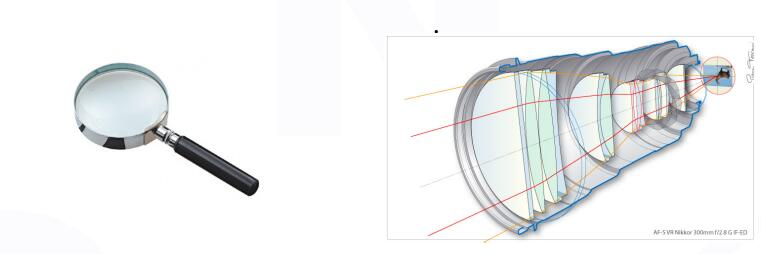
\includegraphics[width=12cm]{Methods/Images/Lenses.jpg} \\
	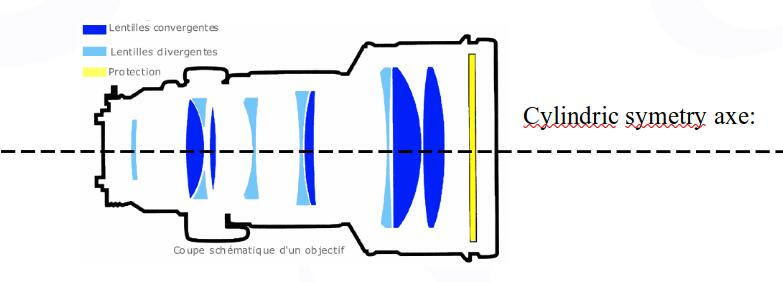
\includegraphics[width=8cm]{Methods/Images/LensesCyl.jpg}
	\caption{A single lense , and modern }
	\label{fig:Lenses}
\end{figure}

We start the modelization with three observations on the theoreticall design of central perspective cameras:

\begin{itemize}
    \item  each individual lense has a radial symetry arround it opticall axe;:
    \item  the mechaninal building is made so that all the lenses are aligned on
	    their common optical axe $\mathcal{A}$.
    \item  the plane of the sensor is orthognal to $\mathcal{A}$.
\end{itemize}

For real camera, these observation are satisfied with a high accurracy in the sense that it is
rigourously satisfied in the theoreticall conception model of almost all central perspective
camera~\footnote{to our knowledge the only notable exception if tilt lenses, for the orthogonality rule}.
Consequently all the corrective terms that we will study in further sections,
are due to the difference between theoreticall model and effective realization and are
generally of an order of magnitude lower than the radial distorsion.

These elementary remarks have for consequence that, how sophisticated may be the combination
of many lenses, each having a complicated non spherical shape, we still have a global cylindrical
symetry on our system. This is illustrated by schemes of figure~\ref{fig:Lenses}.
The perspective center $C$ defined in \ref{Still:Persp}, must belong to the axes of symetry,
so we have $\mathcal{A}=(C,\vec{k})$. 

%--------------------------------------------------------------------------------------------------------

\subsection{Notation}

For a direction of vector we will use spherical coordinates in repair $\vec{i},\vec{j},\vec{k}$ :

\begin{equation}
	\vec{S_{ph}}(\theta,\phi)   =\begin{pmatrix}  \cos(\theta) \sin(\phi) \\ \sin(\theta) \sin(\phi)  \\ \cos(\phi) \end{pmatrix}
	     \label{PC:Spher:Coord}
\end{equation}

We  note $\mathcal{P}_{\theta}$  the plane passing by $\mathcal{A}$ and containing the vector    $\vec{S_{ph}}(\theta,.)$
(the $.$ enhances that whatever may be the value $\neq 0$ , it will define the same plane).

For any ray intersecting $\mathcal{A}$, we will note $R(z,\theta,\phi)$ the ray of direction $\vec{S_{ph}}(\theta,\phi)$  crossing $\mathcal{A}$
at abscissa $z$  :

\begin{equation}
	R(z,\theta,\phi) = \{C+ z \vec{k} + \lambda \vec{S_{ph}}(\theta,\phi), \lambda \in \RR\}
	     \label{PC:RayParam}
\end{equation}


%--------------------------------------------------------------------------------------------------------

\subsection{Intuitive formulation}

Let $B$ be an incoming ray, noted $ R(0,\theta,\phi)$ , let $B'$ be the outcoming ray  that will intersect the sensor,
we want to establish the property of the transformation  $ \Psi : B \rightarrow B'$.
If we admit the \emph{intuitive} following proposals :


\begin{proposal}[3D radial symetry-physicall modelization]  \;
\label{PhysRadMod}
\begin{enumerate}
    \item  $\Psi$ is globally stable inside any plane  $\mathcal{P}_{\theta}$; \label{PhysRadModPlane}

    \item  any  circular cone $\mathcal{C}$ of bundle  arround $\mathcal{A}$ is
	    transformed by $\Psi$ in another circular cone arround $\mathcal{A}$  (but possibly with a different origin and angle);
\end{enumerate}
\end{proposal}

This has for consequence that , noting  $B'=(z',\theta',\phi')$ \footnote{which is possible because $B'$ intersect  $\mathcal{A}$ due to first proposal},
we have : (1) $\theta'=\theta$  (2)  $z'$ and $\phi'$ depends only of $\phi$. 
Then $\Psi $ has the following parametric form, where $\zeta$ and $\Phi$ are mapping $\RR \rightarrow \RR$ :

\begin{equation}
	\Psi(B) = \Psi(R(0,\theta,\phi)) = R(\zeta(\phi) ,\theta,\Phi(\phi))
\end{equation}

Next section is a formal proof,  it can be omited by the reader in a hurry who is already conviced of the above proposal.


%--------------------------------------------------------------------------------------------------------

\subsection{Proof}

\begin{figure}
\centering
	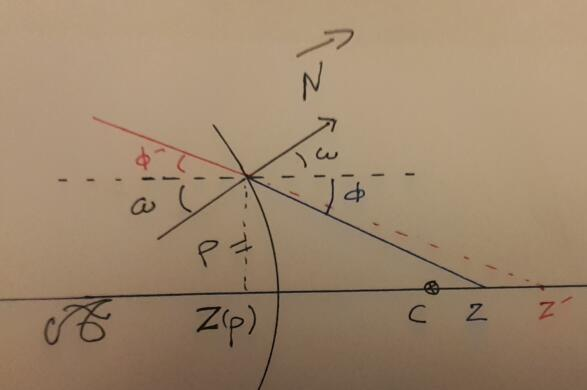
\includegraphics[width=12cm]{Methods/Images/Radial-PhiOmegaZ.jpg} \\
	\caption{Notation for dioptr crossing}
	\label{fig:RadPhiOmegZ}
\end{figure}

The optical system is made of succession of diopters $D_1,\dots D_n$,
that are have all a symetry arround $\mathcal{A}$.  Noting $\Psi_k$
the elementary transformation by a single dioptr  we will  proof ;

\begin{proposal}[3d radial symetry of dioptr]  \;
If  we have a set of ray $R(z,\theta,\phi)$ intersecting  $\mathcal{A}$ such that  z is function of $\phi$ :
$z=\zeta(\phi)$, then  all the output ray satisfy the same property ; they intersect $\mathcal{A}$ and there exist 
two mappings  $\RR \rightarrow \RR$ , $\zeta'$ and $\Phi'$  such:

\begin{equation}
	\Psi(B) = \Psi(R(\zeta{\phi},\theta,\phi)) =  B' = R(\zeta'(\Phi'(\phi)),\theta,\Phi'(\phi))
\end{equation}
\end{proposal}

As the condition \emph{"x is function of $\phi$"} obviously applies for initial rays (i.e. $x=0$ for all as they cross $C$),
we will have proven what we want as $\Psi = \Psi_n \circ  \Psi_{n-1} \circ \dots \circ \Psi_1$. Note also that the requirement
for initial ray is a bit more general than imposing that all ray cross $C$, it is sufficient that they complies with requirement
of proposal above (intersect $\mathcal{A}$ and abscissa of intersection depends only of $\phi$).


We will use cylindric coordinate $\rho,\theta,z$ arround $\mathcal{A}$, where $\theta$ is the same than the spherical
coordinate used in equation~\ref{PC:Spher:Coord}

\begin{equation}
	C_{yl}(\rho,\theta,z)   =\begin{pmatrix} \rho \cos(\theta)  \\ \rho \sin(\theta)   \\ z \end{pmatrix}
	     \label{PC:Cyl:Coord}
\end{equation}

Consider a ray $B$ that is deflected in $B'$ when it meets the dioptr  $D$ in point $P$.
The surface of the dioptr $D$, can be caraterized by the equation $z=Z(\rho,\theta)$, and due to cylindric symetry we have in fact :
$z=Z(\rho)$.  We can then establish a parametric representation of the surface :

\begin{equation}
	Q(\rho,\theta) =  C_{yl}(\rho,\theta,Z(\rho,\theta)) = \begin{pmatrix} \rho \cos(\theta)  \\ \rho \sin(\theta)   \\ Z(\rho) \end{pmatrix}
\end{equation}

The normal $\vec{N}(\rho,\theta) $ to the surface can be computed as :


\begin{equation}
	\vec{N}(\rho,\theta) 
	=  \frac{\partial Q}{\partial \rho} \wedge \frac{\partial Q}{\partial \theta}
	=   \begin{pmatrix} \cos(\theta)  \\  \sin(\theta)   \\    \frac{\partial Z}{\partial \rho}   \end{pmatrix}
            \wedge 
	   \begin{pmatrix} -\rho \sin(\theta)  \\ \rho \cos(\theta)   \\ 0 \end{pmatrix}
	=   \begin{pmatrix}  - \rho \frac{\partial Z}{\partial \rho}  \cos(\theta)  \\  -\rho \frac{\partial Z}{\partial \rho}  \sin(\theta)   \\  \rho     \end{pmatrix}
	=   \begin{pmatrix}  0 \\  0 \\  \rho     \end{pmatrix}
            - \rho \frac{\partial Z}{\partial \rho}   \begin{pmatrix}   \cos(\theta)  \\   \sin(\theta)   \\  0     \end{pmatrix}
		    \label{PC:EqNorm}
\end{equation}

Equation~\ref{PC:EqNorm} shows that the normal  $\vec{N}(\rho,\theta)$ belongs to plane $\mathcal{P}_{\theta}$. 
So as $\vec{N}(\rho,\theta)$ and $\vec{B}$  belongs to $\mathcal{P}_{\theta}$ , first Snell-Descartes law on refraction 
implies that  $\vec{B'}$ belongs also to  $\mathcal{P}_{\theta}$.  This proves the first
that $B' \subset  \mathcal{A}$ and $\theta'=\theta$.

Let write $\vec{N} = S_{ph}(\theta,\omega)$ as illustrated on  figure ???;  due to radial symetry  ,
$\omega$ does not  depends of $\theta$ (see also equation~\ref{PC:EqNorm} : $\tan(\omega)= \frac{\partial Z}{\partial \rho}$) :  $\omega$  depends only of $\phi$.
So using Snell-Descartes law on refraction gives, noting $n$ the reflexion indice after $D_k$, we have :

\begin{equation}
	n'  \sin(\omega + \phi') = n  \sin(\omega + \phi)
\end{equation}

This proves that $\phi'$ is a function of $\phi$ :  $\phi' = \Phi(\phi)$.

Also we have  :


\begin{equation}
	\sin(\phi) = \frac {z-Z(\rho) }{\rho}
	\label{Eq:PhiZRhoIn}
\end{equation}
\begin{equation}
	\sin(\phi') = \frac {z'-Z(\rho) }{\rho}
	\label{Eq:PhiZRhoOut}
\end{equation}

Equation \ref{Eq:PhiZRhoIn} show that $\rho$ is a function of $\phi$  and $z$, then $\rho$ is a function of $\phi$ (as $z$ is function of $\phi$).
Equation \ref{Eq:PhiZRhoOut} show $z'$ is a function of $\rho$ and $\phi'$, but $\rho$ is a function of  $\phi$ and
then a function of $\phi'$  ($\phi = \Phi^{-1}(\phi')$).


%--------------------------------------------------------------------------------------------------------

\subsection{Radial distorsion in the plane}

\begin{figure}
\centering
	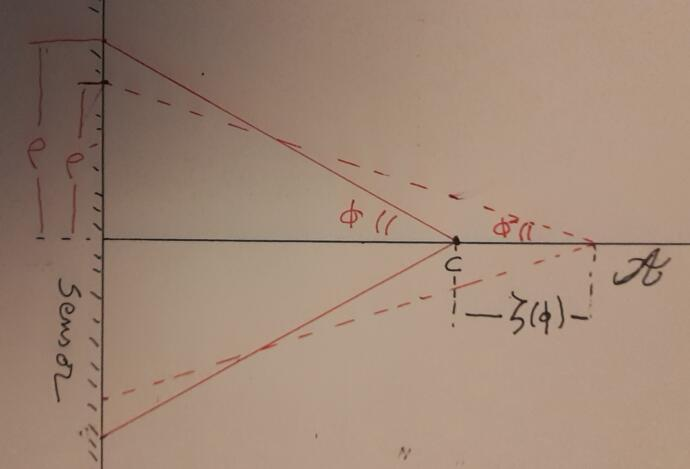
\includegraphics[width=12cm]{Methods/Images/RadialInThePlane.jpg} \\
	\caption{Notation radial distorsion}
	\label{fig:RadInPlane}
\end{figure}

Untill now, we have computed the distorsion in $3d$ as a function $\Psi$ modifying the path of light. To use 
equations~\ref{FormImage1} and~\ref{FormImage2} we need to convert the effect $\Psi$  in image plane.
We use notation of figure~\ref{fig:RadInPlane}.


Without distortion the ray will arrive at point $q$  given by :

\begin{equation}
	q =     \begin{pmatrix} P^p_x \\ P^p_y \end{pmatrix} +  F \tan(\phi)   \begin{pmatrix} \cos(\theta) \\ \sin(\theta) \end{pmatrix} 
\end{equation}

With distorsion, the ray will arrive at point $q' = D(q)$ given by :

\begin{equation}
	q' =     \begin{pmatrix} P^p_x \\ P^p_y \end{pmatrix} +  (F+z') \tan(\phi')   \begin{pmatrix} \cos(\theta) \\ \sin(\theta) \end{pmatrix} 
		=     \begin{pmatrix} P^p_x \\ P^p_y \end{pmatrix} +  (F+\zeta(\Phi(\phi))) \tan(\Phi(\phi))   \begin{pmatrix} \cos(\theta) \\ \sin(\theta) \end{pmatrix} 
\end{equation}

Using polar coordinates arround $P^p$ we have :

\begin{equation}
	q = P^p + P_{ol}(\rho,\theta) =  P^p+  P_{ol} ( F \tan(\phi), \theta) \label{PolInit} 
\end{equation}

\begin{equation}
	q' = P^p+   P_{ol}(\rho',\theta) =  P^p+  P_{ol}( (F+\zeta(\Phi(\phi))) * \tan(\Phi(\phi)), \theta) \label{PolDist}
\end{equation}

So : 

\begin{equation}
       \rho = F \tan(\phi)   \;\;\; , \;\;\;  \rho' = (F+\zeta(\Phi(\phi))) * \tan(\Phi(\phi))   \label{RhoPhi}
\end{equation}

We see that $\rho$ and $\rho'$ are both function of $\phi$, this show that $\rho'$ can be
computed as a function of $\rho$ (just replace $\phi$ by $\tan^{-1}(\frac{\rho}{F})$ in  $\rho'= (F \tan(\phi) +\zeta(\Phi(\phi))) * \tan(\Phi(\phi))$,
\footnote{but the exact formula istself is not important}).
The distorsion $D : q \rightarrow q' $ can then be completely caracterized by the radial distorsion
$D_r : \rho \rightarrow  \rho'$ :

\begin{equation}
	D(q)  =   D(P_{ol}(\rho,\theta))  =   P_{ol}(D_r(\rho),\theta)
\end{equation}

%--------------------------------------------------------------------------------------------------------

\subsection{Polynomial radial distorsion in polar coordinate}

The three point important in formula~\ref{RhoPhi} and the consequence for $D_r$  are :

\begin{itemize}
   \item $\rho$ and $\rho'$ can be computed as \emph{smooth} function of $\phi$; in fact we can 
         consider that the lenses have $\mathcal{C}^{\infty}$ shape ,  then   $\rho$ and $\rho'$ 
         are $\mathcal{C}^{\infty}$ are functions of $\phi$ , and finally $\rho'$ is a 
         $\mathcal{C}^{\infty}$ function $\rho$;

   \item for standard optics we have  $\zeta \approx 0$ and $\Phi \approx Id$,  then we have $D_r \approx Id$;
         by standard standard optics we mean optics where lenses are relatively thin, then  we are not far from Gauss approximation,
         this hypothesis do not hold for fish-eye lenses and we will rediscuss that in section~\ref{SecFE};

   \item $\rho$ and $\rho'$ are  \emph{odd}  function of $\phi$ , and then $\rho'=D_r(\rho)$ is as an \emph{odd}  function of 
        $\rho$;

\end{itemize}

As a synthesis :

\begin{proposal} \;
\label{DrHyp}
       $D_r$ is $\mathcal{C}^{\infty}$, odd function close to identity.
\end{proposal}

For justifying the polynomial approximation of $D_r$, we can then use a classical result of function 
approximation, the Stone-Weierstrass theorem (\cite{Weierstrass1885} and \cite{Stone1937})
which say that the space of polynoms is dense in the space of continuous function on closed bounded set;
so with a sufficient degree the function can be approximated as close as we want by a polynom.
Which lead to the parametric formula for $D_r$ and $D$ :

\begin{equation}
	D_r(\rho)  =   \rho  * (k_0 + k_1 \rho^ 2 + k_2 \rho^4 \dots  + k_n \rho^{2n})
\end{equation}

This formula require several comment :

\begin{itemize}
    \item  as $D_r$ is an odd function, we have only odd degree for polynom ; 

    \item  in the next we will set $k_0=1$, as the variation on scale are already handled by focal;
\end{itemize}

%--------------------------------------------------------------------------------------------------------

\subsection{Polynomial radial distorsion in euclidean coordinates}

Also polar coordinate are convenient for modelization of phenomena with radial symetry, 
they are not ideal for computation : they are relativelly slow and  the center point is
a critical point that can complexify some equation.  Sometime we cannot avoid them
easily, but here it happens that we can express w/o problem the distorsion
with euclidean coordinates:

\begin{equation}
\begin{multlined}
D(q)  =   P_{ol}(\rho  * (1 + k_1 \rho^ 2 + \dots) ,\theta)  \\
=   (1 + k_1 \rho^ 2 +  k_2 \rho^ 4 \dots)  \begin{pmatrix} \rho\cos(\theta) \\ \rho \sin(\theta) \end{pmatrix} \\
=   (1 + k_1 (x^2+y^2) +  k_2 (x^2+y^2) ^2 \dots)  \begin{pmatrix} x \\ y \end{pmatrix}
\end{multlined}
\end{equation}



%--------------------------------------------------------------------------------------------------------

\subsection{Variations on  conventions on radial distorsion}

As often in photogrammetry, there are many conventions and options for representing the same thing,
or small variations on the same things, in different book, papers, software \dots
We discuss here some of this options.

  % -  -  -  -  -  -  -  -  -  -  -  -  -  -  -

\subsubsection{Order of combinaison}

In previous section, in equation~\ref{FormImage2}, we have written  $ \mathcal{I} = \mathcal{I}_0  \circ D \label{FormImage2}$.
In several software the order of combination is invert of this one and authors use instead:

\begin{equation}
	\mathcal{J} = D \circ  \mathcal{I}_0  
\end{equation}

First we can remark that from the mathematicall point of view, the two convention are equivalent in the sense
that they define the same space of function.  With first convention we have :

\begin{equation}
	\mathcal{I}(q) = P^P + F (1 + k_1 (x^2+y^2) +  k_2 (x^2+y^2) ^2 \dots)  \begin{pmatrix} x \\ y \end{pmatrix}
\end{equation}

With second convention , as we operate on pixel the center of radial symetry will  be $P^p$ 
(althouh with "our" convention it is implicitely $0,0$). For the radial distorsion 
we compute first  $  \mathcal{I}_0 : q \rightarrow  P^p + F*q$, then we substract 
$P^p$  who is the center of distorsion, and obtain the formula :

\begin{equation}
	\mathcal{J}(q) = P^P + (1 + K_1 F^2 (x^2+y^2) +  K_2  F^4 (x^2+y^2) ^2 \dots)  \begin{pmatrix} F*x \\ F*y \end{pmatrix}
\end{equation}

So we see that they are equivalent and the conversion is here relatively easy  $K_1 = \frac{k_1}{F^2} $,
$K_2 = \frac{k_2}{F^4} $ \dots

This show  that there is no "hard" reason for selecting one convention to the other. The reason for
prefering convention  $\mathcal{I}_0  \circ D$ was :

\begin{itemize}
    \item some \emph{a priori} preference for numbers without unity;

    \item coefficient easier to interpret (typically, on realistic example, between $10^{-1}$ and $10^{-3}$ rather than between $10^{-8}$ and  $10^{-27}$)

    \item \emph{a priori} better for numerical stability.
\end{itemize}

  % -  -  -  -  -  -  -  -  -  -  -  -  -  -  -

\subsubsection{Names of coefficients}

In computer vision, the coefficient are name $k_1$, $k_2 \dots$ 
In  "traditionnal" photogrammetry, they are often named $R_3,R_5,R_7\dots$.

  % -  -  -  -  -  -  -  -  -  -  -  -  -  -  -

\subsubsection{Degree of polynon}

There is the question of what is the desirable degree of $n$, this is related to the general question issued in~\ref{ParamFit}
and there is no universal answer;  the "tradition" of aerial photogrammetry is to restrict to $n=3$  (i.e. $R_3,R_5,R_7$),
the "tradition" in computer vision is often to restrict to $n=2$, or even $1$;  also with modern lenses and modern
process there is argument for having higer degree  :
           
\begin{itemize}
         \item   with automatic tie point, we have currently several thousand measurement, the risk of over parametrisation
                 with $n=5$ , or even $10$ is low;

         \item   with automatic tie point, we have currently several thousand measurement, the risk of over parametrisation
\end{itemize}

  % -  -  -  -  -  -  -  -  -  -  -  -  -  -  -

\subsubsection{PPA and PPS}

In aerial photogrammetry, the "tradition" is to consider that the center of symetry of radial distortion
is different of principal point; they are named PPA (principal point of autocolimation) and
PPS (principal point of symetry).

We dont do it in {\tt MMVII} because it woul be redundant we other parameters 
selected as discussed in detail in \label{PPA:PPS:DEC}.
This is why in previous section we have used $P^p$ the center of symetry of the distorsion 
(in fact $0,0$ with our conventions).

%-----------------------------------------------------
%-----------------------------------------------------
%-----------------------------------------------------

\section{Decentric distorsion}
\label{DecMod}

\subsection{Introduction}
The previous section has establish the radial distorsion, that would almost always
be sufficient if the physical camera was a perfect realization of the designed camera.
In the next section we will discuss the main "default" in the realisation of
the camera and the additional parameters that are added to modelize them.

The first hypothesis  that will be questionned is the fact that the axes of the different
lenses are perfectly aligned.

%-----------------------------------------------------
\subsection{Mathematicall modelisation}

First we must translate in mathematicall terms the physicall words
"the lenses are slightly miss aligned".
We will do it by  the following assumption :

\begin{itemize}
    \item  each of the $N$ elementary block of well alligned lenses can still be 
           modelized by a central distorsion $D^k$ of centre $C^k$ and radial
           disorsion $D^k_r$;

    \item  the globall distorsion is the composition of the elementary distorsion
           $ D = D^1 \circ D^2 \circ \dots \circ D^n$

    \item  all the elementary distorsion are close to identidy, what we write :
           $D^k = Id + \delta^k$  with $\delta^k \approx 0$;

    \item  all the center of symetry are close to each others , and for simplicity
           we will write $C_k \approx (0,0)$;
\end{itemize}


We first need to show that $D^1 \circ D^2  \approx Id + \delta_1 + \delta_2$ up to second order term.
We will write $A\ll B$ for A is negligible with respect to B. We write $\nabla_F$
the jacobian of $F$, we have the taylor expansion :

\begin{equation}
	F(x+d_x) = F(x) + \nabla_F d_x + \epsilon(|d_x|) |d_x|  \;\; ; \;\;  \epsilon(|d_x|) \ll 1
\end{equation}


Consider now two function close to identity $D^1$ and $D^2$, we can write :
\begin{equation}
\begin{multlined}
(D^1 \circ D^2)(p)  \\
=  (Id+\delta^1)(p+\delta^2(p))\\
=  p +\delta^2(p) + \delta^1(p+\delta^2(p)) \\
=  p +\delta^1(p) + \delta^2(p) + \nabla_{\delta^1} \delta^2   + \epsilon(\delta^2(p)) |\delta^2(p)|
\end{multlined}
\end{equation}

For a firts order approximation of last line :

\begin{itemize}
   \item we have $\epsilon(\delta^2(p)) |\delta^2(p)|  \ll |\delta^2(p)|$ because $\epsilon\ll 1$,
          and this term can be neglected at first order;

   \item  for  $ \nabla_{\delta^1} \delta^2$ , it's less obvious, we admit here that
          if $\delta^1 \ll 1$ then $ \nabla_{\delta^1} \ll 1$,  in fact say like w/o further hypothesis this
		is wrong \footnote{consider for example $x^2 sin(\frac{1}{x})$, but its not $\mathcal{C}^\infty$}, but it becomes
          true if we add the condition that $\delta^1$ is smooth, however this would take us too far  and we admit it;
\end{itemize}

We have shown that $D^1 \circ D^2  \approx Id + \delta_1 + \delta_2$ .  Now it's trivial by recurence to
show that :

\begin{equation}
     D^1 \circ D^2   \dots D^n  \approx Id + \delta^1 + \delta^2 \dots + \delta^n
\end{equation}

%-----------------------------------------------------

\subsection{$2$ block case}

Consider now $D_1$ and $D_2$ two  radial distorsion; using center $C_k$, let write :

\begin{itemize}
	\item $\vec{u}_k = \overrightarrow{C_k p} = ^t (x_k,y_k) $ the vector joining $C_k$ to $p$;
	\item $R_k = ||\vec{u}_k||^2$  the square of the norm of $\vec{u}_k$ (i.e.  square of $\rho_k$ in radial coordinates) ;
\end{itemize}


Using the polynom  of distorsion $D^k_r(R) = k^k_1 R + k^k_2 R^2  \dots$  , we can write :
\begin{equation}
	\delta^k(p) =   D^k_r(R_k) \vec{u}_k 
\end{equation}

Then :

\begin{equation}
\begin{multlined}
	D^1 \circ D^2 (p)  \\
	= p +\delta^1(p) +\delta^2(p) \\
	= p +    D^1_r(R_1) \vec{u}_1  +  D^2_r(R_2) \vec{u}_2  \\
\end{multlined}
\end{equation}

As the two distorsions have close centers, even if their polynom of distorsion funcion are very different,
we can expect that each is close to a radial distorsion with the center of the other.
So we take arbitray one of both as the "reference, here  $D_1$,
and we write $D_2$ as a distorsion around the $C_1$ with polynom of $D^2_r$  plus an corrective term :

\begin{equation}
	\delta^2(p) =   D^r_2(R_1) \vec{u}_1  + ( D^2_r(R_2) \vec{u}_2 - D^2_r(R_1) \vec{u}_1 )
\end{equation}

In this equation the first term is a radial distorsion of center $C_1$. For the second term,
consider the function $\vec{\delta_2}$ defined by :

\begin{equation}
	\vec{\delta^2}(\vec{u}) =  D^r_2(||\vec{u}||^2) \vec{u}
\end{equation}

We can write the second term as :

\begin{equation}
	\vec{\delta^2}(\vec{u_2})  - \vec{\delta^2}(\vec{u_1})
\end{equation}

This term, can then be seen as the difference of the values of function $\vec{\delta^2}$, between $\vec{u_2}$
and $\vec{u_1}$.  But $\vec{u_2}$ and $\vec{u_1}$ are close because
$C_1$ and $C_2$ are. So we can approximate this term with  a Taylor expansion :

\begin{equation}
	\vec{\delta^2}(\vec{u_2})  - \vec{\delta^2}(\vec{u_1})
	\approx
	(C^2_x - C^1_x) \frac{\partial{\vec{\delta^2}}}{\partial x} (\vec{u_1})
     + 	(C^2_y - C^1_y) \frac{\partial{\vec{\delta^2}}}{\partial y}  (\vec{u_1})
\end{equation}

Note that we have used $\vec{u_1}$ as value where the devlopment is made, we could have used $\vec{u_2}$,
it's arbitrary and they are close.
So, merging previous equation, we can write :

\begin{equation}
	D^1 \circ D^2 (p) 
	\approx
	  p +    (D^1_r(R_1) + D^2_r(R_1))  \vec{u}_1  
	  +  \Delta_x \frac{\partial{\vec{\delta^2}}}{\partial x} (\vec{u_1})
          +  \Delta_y \frac{\partial{\vec{\delta^2}}}{\partial y}  (\vec{u_1})
\end{equation}

The term $(D^1_r(R_1) + D^2_r(R_1))  \vec{u}_1 $ is a pure radial term 
(with center $C_1$).    The second term is the "decentric" term itself.
To keep it simple, we will adopt the usual implicit convention for this term,
we limit the radial distosion to the first term $k_1 \rho_1^2$; note that {\tt MMVII} allow to use 
abitrary number of term .  So we have

\begin{equation}
\begin{multlined}
	\vec{\delta^2} (\vec{u_1}) = k_1(x_1^2+y_1^2)  \begin{pmatrix} x_1  \\ y_1 \end{pmatrix} \\
%
		\frac{\partial{\vec{\delta^2}}}{\partial x} 
		=  k_1 \begin{pmatrix} 3 x_1^2 + y_1^2    \\ 2 x_1 y_1  \end{pmatrix}
%
			\;\;\;\;   ; \;\;\;\;   
		\frac{\partial{\vec{\delta^2}}}{\partial y} 
		=  k_1 \begin{pmatrix} 2 x_1 y_1 \\ x_1^2 + 3 y_1^2  \end{pmatrix}
\end{multlined}
\end{equation}


Using standard convention, we name $\alpha = k_1  \Delta_x $ and $\beta = k_1  \Delta_y$;

\begin{equation}
	D^1 \circ D^2 (p) 
	\approx
	= p +    (D^1_r(R_1) + D^2_r(R_1))  \vec{u}_1  
	  +\begin{pmatrix} \alpha(3 x_1^2 + y_1^2 ) +2\beta x_1 y_1   \\ 2  \alpha x_1 y_1 +  \beta( x_1^2 + 3 y_1^2)  \end{pmatrix}
\end{equation}

%-----------------------------------------------------

\subsection{N block case}

We now analyse the case where have more than $2$ block.  


\begin{equation}
\begin{multlined}
	D^1 \circ D^2 \circ D^3 \dots (p)  \\
	= p +\delta^1(p) +\delta^2(p) + \delta^3(p) \dots 
\end{multlined}
\end{equation}

We have :

\begin{equation}
\begin{multlined}
        \delta^k(p)  
	\approx  (D^k_r(R_1))  \vec{u}_1  
          +\begin{pmatrix} \alpha_k(3 x_1^2 + y_1^2 ) +2\beta_k x_1 y_1   \\ 2  \alpha_k x_1 y_1 +  \beta_k( x_1^2 + 3 y_1^2)  \end{pmatrix} \\
\end{multlined}
\end{equation}

Naming $\alpha =  \alpha_1+\alpha_2 + \dots$ and $\beta$ idem we then have again:


\begin{equation}
\begin{multlined}
	D^1 \circ D^2 \circ D^3 \dots (p)  \\
	\approx  p + (D^1_r(R_1) + D^2_r(R_1) +  D^3_r(R_1 \dots )  \vec{u}_1
	  +\begin{pmatrix} \alpha(3 x_1^2 + y_1^2 ) +2\beta x_1 y_1   \\ 2  \alpha x_1 y_1 +  \beta( x_1^2 + 3 y_1^2)  \end{pmatrix}
\end{multlined}
\end{equation}

So we see that, to the first order, any combination of radial distorsion with slightly different centers,
can be approximated by a \emph{unique} radial distorsion plus a decentric distorsin parametrized by the two value $\alpha,\beta$.

%-----------------------------------------------------
%-----------------------------------------------------
%-----------------------------------------------------

\section{Calibration as mapping "up to a rotation"}

\subsection{Introduction}

Before going deeper in the progressive refinement in modelisation of
distorsion, we  make a preliminary remark that is important
to avoid over parametrization (we do it now because, this over parametrisation
does not occurs this model previously described in~\ref{RadMod} or~\ref{DecMod}).


The function $\mathcal{I} \circ \pi_0$  of equation~\ref{FormImage1} can be seen as a function that
goes from the sphere of direction to the sensor.  In a first
step we will show that this determination of this function is intrinsequely ambiguous
\emph{up to a rotation} and then we will see the consequences.


\subsection{Setting equations}

In equation ~\ref{FormImage1} , we note :

\begin{equation}
	P-C =  \overrightarrow{CP}  = \begin{pmatrix} x_c \\ y_c \\ z_c \end{pmatrix} 
\;\;\;  ;  \;\;\;
        ^t R =  \begin{pmatrix}  A & B & C \\ D & E & F \\ G & H & I \end{pmatrix} 
\end{equation}

Now we have in equation~\ref{DecMod} :

\begin{equation}
	\pi_0(^t R(\overrightarrow{CP})) 
	=  \frac{\begin{pmatrix} Ax_c+By_c+Cz_c \\ Dx_c+Ey_c+Fz_c  \end{pmatrix}}{Gx_c+Hy_c+Iz_c}
		=  \frac{\begin{pmatrix} A\frac{x_c}{z_c}+B\frac{y_c}{z_c}+C \\  D\frac{x_c}{z_c}+E\frac{y_c}{z_c}+F  \end{pmatrix}}
			{G\frac{x_c}{z_c}+H\frac{y_c}{z_c}+I}
\end{equation}

Let note $H_R$ the $2D$  homography defined by :

\begin{equation}
 H_R(u,v) =  \frac{\begin{pmatrix} Au+Bv+C \\  Du+Ev+F  \end{pmatrix}} {Gu+Hv+I}
\end{equation}

We then have :

\begin{equation}
	\pi_0(^t R(\overrightarrow{CP}))  = H_R  (\pi_0 (\overrightarrow{CP}))
\;\;\;  ;  \;\;\;
        \pi_0  \trans  R = H_R  \pi_0
\end{equation}

We now go back to equation~\ref{FormImage1}, and for any rotation $R'$, we insert it using $^t R'R'=Id$ :

\begin{equation}
	\mathcal{I} \pi_0   \trans R = \mathcal{I}  \pi_0   (\trans R' R')  \trans R = ( \mathcal{I}  \pi_0   \trans R')  (R' \trans R )
\end{equation}

We finally have :

\begin{equation}
	   \mathcal{I} \pi_0   \trans R 
	   = (\mathcal{I} H_{R'})   \pi_0   \trans (R \trans R')  \label{FormRotCalib}
\end{equation}


%-----------------------------------------------------

\subsection{Interpretation}

The interpretation of equation~\ref{FormRotCalib} is the following : 

\begin{proposal}[Pose/calibration mixing]  \;
A camera with
a calibration $\mathcal{I}$ and pose $(R,C)$ has exactly the same projection
function that a camera with calibration $\mathcal{I} H_{R'}$ and pose $(R \trans R',C)$ where $R'$
is an arbitrary rotation.
\end{proposal}

The consequence of this proposal is that if $\mathcal{I}$ is a "valid" calibration of the
camera, then for any rotation $R$,  $\mathcal{I} H_{R}$ is also a valid calibration.
Intuitively, we see that this may create difficulties and over parametrization when
 $\mathcal{I} H_{R}$ belongs to the model we try to compute.

The importance of this remarks depends of the model of distorsion we have selected.
We some model if $\mathcal{I}$ is a valid distorsion,  $\mathcal{I} H_{R}$ will
never be a valid distorsion (except with trivial case $R=Id$) and we dont need
to take precaution.

%-----------------------------------------------------

\subsection{Intuitive analyse of dangerous case}

\begin{figure}
\centering
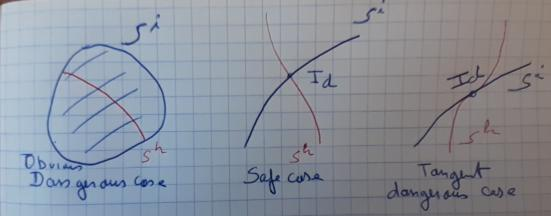
\includegraphics[width=12cm]{Methods/Images/TangentSpace.jpg}\caption{Possible relations between $\mathcal{S}^h$ and $\mathcal{S}^i$}
	\label{fig:TanSpace}
\end{figure}


Let notes  $\mathcal{S}^i$ the functionnal space of parametric function  that are selected
for coding functions $\mathcal{I}$, and $\mathcal{S}^h$ the space of all $H_R$ for
$R$ parsing the space of rotation.
The figure~\ref{fig:TanSpace} represent symbolicly the possible relations between
$\mathcal{I}$, and $\mathcal{S}^h$.  Note that this figure is just an
abstraction because in general $\mathcal{S}^i$ will be a high dimensionnal
vectorial space \footnote{for example, $8$ with $PP,F,k_1,\dots\alpha$} 
and  $\mathcal{S}^h$  is a $3$ dimensionnal manifold.

$\mathcal{S}^h$ and $ \mathcal{S}^i$  both contain identity  : $Id \in \mathcal{S}^h \cap \mathcal{S}^i$. 

An obvious dangerous case is symbolized by left image of
figure~\ref{fig:TanSpace},  it is when $\mathcal{S}^h \subset \mathcal{S}^i$ .
An almost identicall dangerous case is when a non trivial subset of $\mathcal{S}^h$
is included in  $\mathcal{S}^i$.

is obviously a dangerous case for computing 
calibration because we will have an infinite number of solution. This would be the case
with universal model where distorsion are considered to be any smooth function.



Generally we will solve this difficulty by restrincting to an "adequate" subset of  $\mathcal{S}^i$ .


Another obvious case occurs when  $\mathcal{S}^h \cap \mathcal{S}^i \neq \{Id\}$

The case where  $\mathcal{S}^h \cap \mathcal{S}^i =\{Id\}$



%-----------------------------------------------------
%-----------------------------------------------------
%-----------------------------------------------------

\section{Sensor inclination}

%-----------------------------------------------------

\subsection{physicall modelisation}

\begin{figure}
\centering
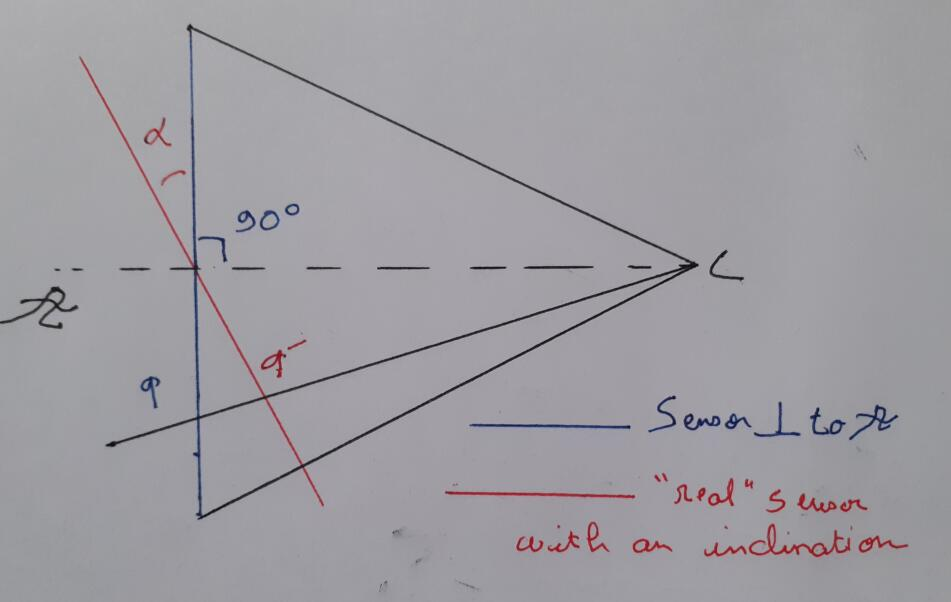
\includegraphics[width=12cm]{Methods/Images/PlanIncl.jpg}\caption{Notation for sensor inclination}
	\label{fig:PlaneIncl}
\end{figure}

The secons hypothesis  that will be questionned is the fact that the sensor is 
orthogonal to axes $\mathcal{A}$.  Using the notation illustatred by 
figure \ref{fig:PlaneIncl}, we will proceed this way :

\begin{itemize}
    \item consider a "theoricall" camera with a sensor orthognal to $\mathcal{A}$ (blue on figure \ref{fig:PlaneIncl});

    \item consider a "real" camera with a sensor tilted (in red);

    \item with consider that rotation is done arround $P^p$, because any global translation of the sensor
         would lead to variation of focal that are already modelized;

    \item  for a given ray, let $q$  be the point that intersect the  orthogonal plane,
	    and $q'$ the point that intersect the tilded  plane, we note
           $\mathcal{T}$  the mapping $\mathcal{T} : q \rightarrow q'$.

\end{itemize}

We will assume that the distorsion $D^t$ of the tilted camera is the combination
of the distorsion of untilted camera and $\mathcal{T}$ :

\begin{equation}
	D^t = \mathcal{T} \circ D 
\end{equation}

%-----------------------------------------------------

\subsection{mathematicall modelisation}

For now we make the hypothesis that the tilt is made by a rotation of angle $\alpha$ arround axe $(O\vec{i})$.
Let $\mathcal{P}_\alpha$ the plane we obtain.  We can compute a basis  of $\mathcal{P}_\alpha$ defines
by  $\vec{i} $ and  $\vec{j}_\alpha $


\begin{equation}
	\vec{j}_\alpha = \begin{pmatrix} 0 \\ \cos(\alpha) \\ \sin(\alpha)  \end{pmatrix}
\end{equation}

To compute the coordinate of $q'$, we use the fact that $q,q',C$ are aligned and $q' \in \mathcal{P}_\alpha$ :

\begin{equation}
        \lambda \begin{pmatrix} x \\ y  \\ 1  \end{pmatrix}
      = x'  \vec{i} + y' \vec{j}_\alpha  + \vec{k}
      =	\begin{pmatrix} x' \\ y'\cos((\alpha)  \\ 1+y'\sin((\alpha)  \end{pmatrix}
\end{equation}


The we compute ratio :

\begin{equation}
	\frac{y'\cos(\alpha)}{1+y'\sin(\alpha)} =  y \;\;\; ; \;\;\;  
	\frac{x'}{y'\cos(\alpha)} =  \frac{x}{y} 
\end{equation}

And solve the equation :

\begin{equation}
	y' = \frac{y}{\cos(\alpha) -y \sin(\alpha)} =  y \;\;\; ; \;\;\;
	x' = \frac{x}{1-y \tan(\alpha)}
\end{equation}



%-----------------------------------------------------
%-----------------------------------------------------
%-----------------------------------------------------

\section{"Universal" model}

\subsection{Assemblage camera}
\subsection{$360$ camera}

\section{Fish eye model}
\label{SecFE}

\section{Note and PPA , PPS and decentric dist}
\label{PPA:PPS:DEC}


\section{Note work to do on non perspective camera}



%-----------------------------------------------------
%-----------------------------------------------------
%-----------------------------------------------------





